\documentclass[12pt]{article}

\usepackage[dvips,letterpaper,margin=0.75in,bottom=0.75in]{geometry}
\usepackage{cite}
\usepackage{slashed}
\usepackage{graphicx}
\usepackage{amsmath}
\usepackage{braket}
\usepackage{latexsym,amssymb,amsmath}
\usepackage{pdfpages}
\usepackage{xcolor}

\usepackage[american,fulldiode]{circuitikz}
\tikzset{component/.style={draw,thick,circle,fill=white,minimum size =0.75cm,inner sep=0pt}}

\begin{document}
\ctikzset{bipoles/thickness=1}
\ctikzset{bipoles/length=.6cm}

\title{Proposal for Revising the \\ Undergraduate Physics Curriculum \\ Version 1.6}
\author{Undergraduate Curriculum Committee}

\maketitle

\section{Objectives of the Proposal}

\begin{table}
\caption{An example schedule for an undergraduate physics major that takes the 9H series and 122A. Physics course numbers are shown with the number of units in parenthesis.  Math courses start with M.  Taking MAT 21A in fall is also common with instructor permission, with MAT 21D taken over the summer to catch up in time for 9HD.  Courses in italics are electives or have at least two different offerings per year. Course CS is a capstone elective, and course X is any advanced elective.}

\label{tbl:current-honors}
\begin{center}
\begin{tabular}{|l|l|l|l|}
\hline
Year      & Fall    & Winter & Spring \\
\hline
Freshman  & 9HA(5)     & 9HB(5)     & 9HC(5) \\
          & {\it M21B(4)}  & {\it M21C(4)}  & {\it M21D(4)} \\
\hline
Sophomore & 9HD(5)     & 9HE(5)     & 40(4)     \\
          & {\it M22A(3)}     & {\it M22B(3)} & {\it 80(4)} \\
\hline
Junior    & 104A(4) & 105B(4) & 110B(4)\\
          & 105A(4) & 110A(4) & 115A(4)\\
          & 102(1)  &    &     \\
\hline
Senior    & 110C(4) & {\it 122A(4)} & {\it X(3-4)}\\
          & 112(4)  & {\it CS(4)}   & {\it X(3-4)}\\
          & 115B(4) & {\it CS(4)}   & {\it CS(4)}\\

\hline 
\end{tabular}
\end{center}
\end{table}

\begin{table}
\caption{An example schedule for undergraduate physics major that transfers to UC Davis in their junior year and takes 122A.  Physics course numbers are shown with the number of units in parenthesis.  Courses in italics are electives or have at least two different offerings per year.  Course CS is a capstone elective, and course X is any advanced elective.}
\label{tbl:current-transfers}
\begin{center}
\begin{tabular}{|l|l|l|l|}
\hline
Year      & Fall    & Winter & Spring \\
\hline
Junior    & 9D(4)   & 105B(4) & 40(4)   \\
          & 104A(4) & 110A(4) & 110B(4) \\
          & 105A(4) & {\it 80(4)}   & 115A(4) \\
          & 102(1)  &         & \\
\hline
Senior    & 110C(4) & {\it 122A(4)} & {\it X(3-4)}\\
          & 112(4)  & {\it CS(4)}   & {\it X(3-4)}\\
          & 115B(4) & {\it CS(4)}   & {\it CS(4)}\\
\hline 
\end{tabular}
\end{center}
\end{table}


An example schedule of student coursework is shown in Table~\ref{tbl:current-honors} for students taking Honors Physics.  An example schedule for students that transfer to UC Davis for their junior year is shown in Table~\ref{tbl:current-transfers}.  There are many different trajectories through our program, but most are some variation on these two.  
For consistent comparisons, all the example schedules in this proposal assume the students take 122A and one capstone course in the winter, and two capstone courses in the spring.  Many other lab courses and offerings are possible. There are some deficiencies in the current course of study:
\begin{itemize}
\item Physics majors that complete 9HD or 9D in the fall of their sophomore year have little to do for the rest of the year.  The honors sequence has 9HE, but this is effectively an elective and does little to further prepare students for upper division coursework.  The recent addition of 40 and 80 is helpful in that it provides something for students to do during this time, but the problem still remains that they do not make progress on the upper division core coursework, and 80 is not taken by all students.  The result of this stalling is that the junior and senior year are a race to complete the degree requirements, leaving very little flexibility or time for advanced electives.

\item Students that transfer to UC Davis for their junior year face a wall of coursework that they have to handle in the first quarter: math methods, mechanics, and modern physics.  Many also take 102, which is nominally a one-unit course, but generally nearly as much work as a four-unit course.  For many students, these are the first courses they encounter that require solving challenging homework problems, and they face effectively 16 units.  We have two trains of students running through our program and the fall of their junior year is the train wreck where they collide.

\item The current curriculum does not include sufficient computing practice for our students.  It is useful to consider what a physics degree would look like if we taught calculus the same way we teach computing.  Students would arrive their freshman year and take an introductory calculus course.  Then, they would take their physics courses, which would never mention calculus.  At some point in their junior or senior year, they would take a one quarter course called ``Calculus in Physics'' which would attempt to show all the ways we use calculus in physics.  Our students are experts at calculus because they learn how to use the tool, and then apply it, again and again, throughout their coursework.  To remain relevant in the modern world (or even the world from 20 years ago) our majors need more practice in the use of computing as an essential tool for solving physics problems.

\item Four-year students typically graduate with around 180 units.  Within the College of Letters and Science, we are allowed to require a maximum of 110 units in our majors.  
The current BS physics major requires a minimum of 108 units to complete.  Fitting the canon of undergraduate physics into such a tight space is extremely challenging.  Students complain that we waste time teaching some topics again and again (e.g. Special Relativity from scratch) while completely dropping other topics (e.g. Classical Hamiltonians).  The problem is particularly acute for applied physics majors, where core material must be dropped to make space for coursework outside of physics.

\item The prerequisite structure of the upper division courses creates many tiers.  
As an extreme example, 122 requires 112, which requires 115A, which requires 104A and 105A, both of which require the 9 series.  This, combined with the rapid pace, leaves very little flexibility for students once they start their junior year.  For example, missing any of the four-unit courses in the junior year of Table~\ref{tbl:current-honors} requires an exception to prerequisites or an extra year to graduate.
\end{itemize}
This proposal aims to make significant improvements on each of these issues.

\newpage

\section{Proposed BS Requirements}

The proposed required courses for a BS in physics are presented in Tables~\ref{tbl:prep} and \ref{tbl:core}.  Example schedules are presented in Tables~\ref{tbl:proposed-honors}-\ref{tbl:proposed-transfers}.  The current BS physics major requires a minimum of 108 units.  The proposed BS physics major requires a minimum of 110 units, the maximum allowed by the college.  

\begin{table}
\caption{\label{tbl:prep}Preparatory Subject Matter}
\noindent
\vskip 0.25cm
Units:  53-54. *: recommended, C: concurrently.\\
\begin{tabular}{|llllll|}
\hline
Course & & Units & Offered & Prereqs & Name \\
\hline
MAT & 21A & 4 & FWS & & Differential Calculus\\ 
    & 21B & 4 & FWS & 21A & Integral Calculus \\ 
    & 21C & 4 & FWS & 21B & Partial Derivatives and Series\\ 
    & 21D & 4 & FWS & 21C & Vector Analysis\\ 
    & 22A & 3 & FWS & 21C & Linear Algebra\\ 
    & 22B & 3 & FWS & 22A & Differential Equations\\ 
\hline
\hline

]PHY & 9A & 5 & FS & 21B & Classical Physics {\it (Class. Mech.)}\\ 
    & 9B & 5 & FW & 9A,21C & Classical Physics {\it (Waves, Thermo., Optics.)}\\ 
    & 9C & 5 & WS & 9B,21D & Classical Physics {\it (Elec. and Magn.)}\\ 
    & 9D & 4 & FS & 9C,22A & Modern Physics {\it (Rel. and Quant. Mech.)}\\ 
\hline
&or&&\\
\hline
PHY & 9HA & 5 & F & C:21B/21M & Honors Physics {\it (Class. Mech.)}\\ 
    & 9HB & 5 & W & 21B/21M & Honors Physics {\it (Rel. and Stat. Mech.)}\\ 
    & 9HC & 5 & S & 21C & Honors Physics {\it (Waves and Quant. Mech.)}\\ 
    & 9HD & 5 & F & 21D & Honors Physics {\it (Elec. and Magn.)}\\ 
\hline
\hline
PHY & 40  & 4 & F & & Introduction to Physics Computation \\ 
    & 45  & 4 & W & 40,9D/9HD     & Computational Physics\\ 
    & 80  & 4 & WS & 40,9C/9HD     & Experimental Techniques \\
PHY & 185* & 1 & S & & \\ 
    & 190* & 1 & F & & \\ 
\hline
\end{tabular}
\end{table}

\begin{table}
\caption{\label{tbl:core}Core Subject Matter}
\noindent
\vskip 0.25cm
Units:  42-46. *: recommended, C: concurrently.\\
\begin{tabular}{|llllll|}
\hline
Course & & Units & Offered & Prereqs & Name \\
\hline
PHY & 104A & 4 & F & 9D/9HD,MAT 22B & Mathematical Physics \\ 
    & 105A & 4 & W & 9D/9HD,C:MAT 22B   & Classical Mechanics I\\
    & 105B & 4 & S & 105A,45      & Classical Mechanics II\\ 
    & 110A & 4 & W & 104A         & Electricity and Magnetism I\\
    & 110B & 4 & S & 110A         & Electricity and Magnetism II\\
    & 112  & 4 & F & 104A         & Thermodynamics and Stat. Mech.\\    
    & 115A & 4 & F & 104A,105A    & Quantum Mechanics I \\
    & 115B & 4 & W & 115A         & Quantum Mechanics II \\
    & 115C & 4 & S & 115B,45      & Applications of Quantum Mechanics\\ 
\hline
\hline
PHY & 116A & 4 &  F & 80   & Instrumentation with Discrete Elec.  \\
    & 116B & 4 &  W & 80   & Instrumentation with Integrated Elec.\\ 
\hline
    & or & & & & \\
\hline
PHY & 122A/B & 4 & WS & 80,104A,105A,110B & Advanced Physics Laboratory \\  
    &  & & & \& C:112 C:115A&  \\  

\hline
\hline
 & Any two of & & & & (all three recommended): \\
\hline 
PHY & 110L & 1 & S & 45,C:110B & Comp. Lab in Electricity and Magn. \\
    & 112L & 1 & F & 45,C:112  & Comp. Lab in Statistical Mechanics \\ 
    & 115L & 1 & W & 45,C:115B & Comp. Lab in Quantum Mechanics \\ 
\hline
\end{tabular}\\ \vskip 0.25cm
\noindent
{\bf Electives:} Additional electives to bring the total number of 3-4 unit upper division courses to 14, including at least three from capstone courses.  
(3-4 courses, totaling 12-16 units with current offerings)
\\
\noindent
{\bf Total Units:} 110-112
\end{table}

\begin{table}
\caption{
An example schedule for an undergraduate physics major that takes the 9H series and 122A. Physics course numbers are shown with the number of units in parenthesis.  Math courses start with M.  Courses in italics are electives or have at least two different offerings per year. Course CS is a capstone elective, and course X is any advanced elective.  Rate is 5-9 physics units per quarter.}
\label{tbl:proposed-honors}
\begin{center}
\begin{tabular}{|l|l|l|l|}
\hline
Year      & Fall    & Winter & Spring \\
\hline
Freshman  & 9HA(5)       & 9HB(5)        & 9HC(5) \\
          & {\it M21B(4)} & {\it M21C(4)}  & {\it M21D(4)}\\
\hline
Sophomore & 9HD(5)       & 105A(4)      & 105B(4) \\
          & {\it M22A(3)} & {\it M22B(3)} & {\it 104A(4)} \\
          & 40(4)        & 45(4)       & {\it 80(4)}  \\
\hline
Junior    & 115A(4) & 115B+L(5)  & 115C(4)\\
          & 112+L(5)  & 110A(4)  & 110B+L(5)\\
\hline
Senior    & {\it X(3-4)} & {\it 122A(4)} & {\it CS(4)} \\
          &              & {\it CS(4)} & {\it CS(4)} \\

\hline  
\end{tabular}
\end{center}
\end{table}

\begin{table}
\caption{
An example schedule for an undergraduate physics major that takes the 9 series and 122A. Physics course numbers are shown with the number of units in parenthesis.  Math courses start with M.  Courses in italics are electives or have at least two different offerings per year. Course CS is a capstone elective, and course X is any advanced elective.  Rate is 0-13 physics units per quarter.}
\label{tbl:proposed-nonhonors}
\begin{center}
\begin{tabular}{|l|l|l|l|}
\hline
Year      & Fall    & Winter & Spring \\
\hline
Freshman  & {\it M21A(4)}  & {\it M21B(4)}  & {\it M21C(4)}\\
          &               &               & {\it 9A(5)} \\
\hline
Sophomore & {\it M21D(4)}  & {\it M22A(3)}  & {\it M22B(3)}\\ 
          & {\it 9B(5)}    & {\it 9C(5)}    & {\it 9D(4)} \\
          & 40(4)          &                & {\it 80(4)} \\
\hline
Junior   & {\it 104A(4)}   & 105A(4)       & 105B(4) \\
         & {\it X(3-4)}      & 110A(4)       & 110B+L(5) \\         
         &                 & 45(4)         & \\

\hline
Senior   & 115A(4)    & 115B+L(5)      & 115C(4) \\
         & 112+L(5)   & {\it 122A(4)} & {\it CS(4)} \\
         &            & {\it CS(4)}   & {\it CS(4)}  \\
\hline 
\end{tabular}
\end{center}
\end{table}

\begin{table}

\caption{An example schedule for an undergraduate physics major that 
transfers to UC Davis in their junior year, without Physics 9D or 40 equivalents, and takes 122A. Physics course numbers are shown with the number of units in parenthesis.  Courses in italics are electives or have at least two different offerings per year. Course CS is a capstone elective, and course X is any advanced elective.
Rate is 12-13 units per quarter.}
\label{tbl:proposed-transfers}
\begin{center}
\begin{tabular}{|l|l|l|l|}
\hline
Year      & Fall    & Winter & Spring \\
\hline
Junior   & 9D(4)         & 105A(4)   & 105B(4) \\
         & 40(4)         & 110A(4)   & 110B+L(5) \\         
         & {\it 104A(4)} & 45(4)     & {\it 80(4)} \\
\hline
Senior   & 115A(4)    & 115B+L(5)      & 115C(4) \\
         & 112+L(5)   & {\it 122A(4)} & {\it CS(4)} \\
         & {\it X(3-4)} & {\it CS(4)}   & {\it CS(4)}  \\
\hline 
\end{tabular}
\end{center}
\end{table}

A primary feature of this proposal is that incoming transfer students now overlap in some courses with sophomores that took the honors physics sequence.  This eliminates the stalling of our four-year students while relieving some of the intense academic pressure on incoming transfer students.  Our experience has been that the best of the transfer students perform as well as our four-year students once they have sufficient time to adjust, and this proposal gives them that time.  Accelerating students that took the honors sequence also provides tremendous additional flexibility to their schedule.  

Transfer students that wish to complete their degree in two years are still highly constrained, but instead of facing what amounts to 12 units of upper division coursework upon arrival they now start with four upper division units.  Take the time to compare fall quarter of the junior year in Tables~\ref{tbl:current-transfers} and \ref{tbl:proposed-transfers}, this is a major feature of this proposal.  This gentle introduction does not come at the cost of dramatically increased unit loads later on: transfer students can still complete the degree without exceeding 13 units of physics coursework in any quarter.  

Several new classes have been added, others require changes to their content or will no longer be required:
\begin{itemize}
\item 9A-D and 9HA-D are largely unchanged, however, some fine adjustments may be needed to ensure that the 9 series plus 104A are sufficient preparation for 112.  Also, there are some minor adjustments to the math prerequisites.

\item 9HE is no longer offered.  This course is effectively an elective, with content that varies from instructor to instructor.  By removing it, we allow the students in the honors sequence to start toward the core material sooner, leaving more time for advanced electives. With more relaxed schedule in their senior year, it seems highly plausible that physics majors will take more advanced electives.

\item 45:  This new four-unit course, Computational Physics, will have the 9 series and 40 as prerequisites and will replace the requirement for 102 or 104B.  
The focus will be on solving physics problems at the conceptual level of the 9 series using computational physics.  This course will play an integral role in this revised curriculum and so the content and tools will need to be more consistently covered than in 104B.  

\item 104A:  This course will now be offered in both fall and spring, as discussed further in the discussion of prerequisites.  Most students taking Honors Physics will take the course in the spring, while most transfer students will take the course in the fall.  Two offerings will remove the bottleneck, result in smaller class sizes, and will allow the course to be pitched slightly differently in these two quarters, to better reflect student preparation.

\item 105:  The timing of the 105AB sequence is adjusted to start in winter, and the content of 105A should be adjusted to include all prerequisite material for 115A.  The content of 105AB should be at a level appropriate for a sophomore completing 9HD in Fall.  There is no prerequisite for 104A, but typically students will take 104A either concurrently with 105B or before 105A.

\item 110:  The present curriculum devotes three quarters of required upper division coursework to Electricity and Magnetism (110ABC) compared to two quarters for Quantum Mechanics (115AB).  This proposal removes 110C from the requirements for a BS.  The current sequence covers all of Griffiths.  We could either eliminate 110C entirely and cover a subset of Griffiths in 110AB, or leave the courses as they are and demote 110C to an elective.

\item 112:  The 115A prerequisite for 112 has been removed, and the treatment must rely on quantum from the 9 series instead.

\item The 115 sequence will be extended to a three quarter sequence 115ABC, but some majors will not be required to take 115C.  The prerequisites are 104A and 105A.
The last quarter, 115C, adds 45 as a prerequisite, and the treatment should include extensive computational problems.  The extra time should also allow coverage of new elective topics (for example Quantum Information Theory).  In this version of the proposal, 115C is required for BS physics majors, but this course could be demoted to an elective for all majors to achieve more flexibility.

\end{itemize}

As part of the implementation of this proposal, we should provide suggested textbooks and week-by-week syllabi for the core courses, at a minimum  40, 45, 80, 104A, 105AB, 110AB, 112, and 115AB.

This proposal is approximately neutral with respect to the cost of instruction if we assume that the cost of electives is held constant (we of course have no obligation to do so.)  The second offering of 104A, the new required course 45, the new required course 115C, and the new required one unit computing labs add a total of four new instructors.  But dropping required courses 9HE, 102, 104B and 116C frees 3.3 instructors, for a net increase of 0.7 instructors.  This increase might be higher if the need for more sections of 80 increases the number of instructors needed (currently typically two, although three were initially planned for 2020-2010).  If 115C is an elective, the proposal becomes net negative by 0.3 instructors.  

\section{Computational Physics}

One of the major objectives of this proposal is to better integrate computational physics throughout the curriculum, and this is accomplished in a number of ways:
\begin{itemize}

\item 40:  In response to the ECS department's decision to no longer offer ECS 30, a one quarter introduction to C without any prerequisites, we replaced this required course with own version, PHY 40, in 2018.  This course introduces the computing tools we expect students to use throughout their coursework:  C++ and python.  The problems used to learn the languages are from computational physics, but the primary aim of this course is for students to rapidly learn the basics of programming.

\item 45:  A new four unit computational physics course, PHY 45, replaces the requirement for 102 or 104B.  This course has the 9 series and 40 as prerequisites and will emphasize the algorithms and techniques used in computational physics with extensive computational problem solving.  Because 102 was (technically!) only a one-unit course, this requirement adds three additional units to our requirements, which must be offset by dropping another requirement.

\item Physics 80 is a new lab course introduced in 2018 which includes extensive use of scientific python for data analysis and presentation.  In this proposal, 80 is required for all majors and adds 40 as a prerequisite.

\item There are three new one-unit computational lab courses (110L, 112L, and 115L) designed to be taken concurrently with 110B, 112, and 115B. They are computational problem solving labs related to E+M, thermodynamics, and quantum mechanics.  The emphasis will be on solving problems from upper division physics using computing at the level of PHY 45.
The instructor will present a technique and problem during a single one hour lecture, and the students will have the rest of the week to complete the assignment. 
It is expected that one instructor will teach all three in a single year, which will count as one course.  Each course is offered in a different quarter, so students get three units of computational problem-solving spread across an entire year.  Due to unit limits, we only require two of these courses, but all three are recommended.

\item PHY 105B and 115C have 45 (computational physics) as a prerequisite and
will include extensive computational problem solving as an integral part of the course.
\end{itemize}
Physics BS majors will now be required to take 22 units of coursework that involves extensive computing exercises.  Furthermore, with student computing abilities on more solid ground, capstone and advanced elective courses are likely to evolve to include additional computing exercises and add 45 as a prerequisite.

\section{Lab Coursework}

Physics 80 was introduced in 2018, and is currently a prerequisite for 122A and 122B.  It is anticipated that this will relieve some of the intense time pressure in 122.  In this proposal, Physics 80 is added as a prerequisite for the 116 (Instrumentation) sequence as well.  Physics 80 covers some of the content in current versions of 116A (passive analog electronics) and 116C (computation with scientific python and statistical analysis).  Therefore, the three quarter 116 sequence (A,B, and C) becomes a two quarter sequence, with 116A covering discrete electronics (analog and digital), and 116B covering integrated electronics (microprocessors and FPGAs).  For additional flexibility, 116B no longer has 116A as a prerequisite, as sufficient analog electronics is covered in 80 for the purposes of integrated electronics.  

Physics 80 and 116 share the same dedicated lab space.  The primary time for taking 80 will be in spring quarter, while 116A and 116B will be offered in fall and winter.  This will allow us to offer up to four sections of 80 during prime time in the spring.

\section{Prerequisites}

\begin{figure}
\begin{center}
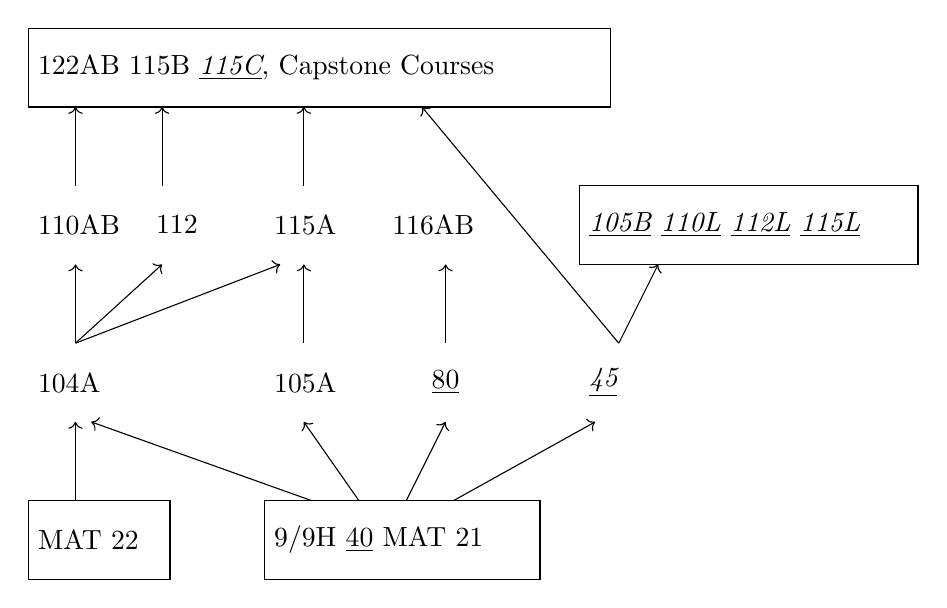
\begin{tikzpicture}

% 1st tier:
\node[right] at (0,0.5) {MAT 22};
\draw (0,0) coordinate(X) -- ++(0,1) -- ++(1.8,0) |- (X);

\node[right] at (3,0.5) {9/9H \underline{40} MAT 21};
\draw (3,0) coordinate(X) -- ++(0,1) -- ++(3.5,0) |- (X);



\draw[->] (0.6,1) --(0.6,2);
\draw[->] (3.6,1) --(0.8,2);
\draw[->] (4.2,1) --(3.5,2);
\draw[->] (4.8,1) --(5.3,2);
\draw[->] (5.4,1) --(7.2,2);
%\draw[->] (7.4,1) --(7.4,2);
%\draw[->] (7.2,1) --(5.5,2);


% 2nd tier:
\node[right] at (0,2.5) {104A};
%\draw (0,2) coordinate(X) -- ++(0,1.0) -- ++(1.2,0) |- (X);

\node[right] at (3,2.5) {105A};

\node[right] at (5,2.5) {\underline{80}};

\node[right] at (7,2.5) {\it \underline{45}};



\draw[->] (0.6,3) --(0.6,4);
\draw[->] (0.6,3) --(1.7,4);
\draw[->] (0.6,3) --(3.2,4);

\draw[->] (3.5,3) --(3.5,4);

\draw[->] (5.3,3) --(5.3,4);

\draw[->] (7.5,3) --(5,6);
\draw[->] (7.5,3) --(8.0,4);


% 3rd tier:
\node[right] at (0,4.5) {110AB};

\node[right] at (1.5,4.5) {112};

\node[right] at (3,4.5) {115A};

\node[right] at (4.5,4.5) {116AB};

\node[right] at (7,4.5) {\it \underline{105B} \underline{110L} \underline{112L} \underline{115L}};
\draw (7,4) coordinate(X) -- ++(0,1) -- ++(4.3,0) |- (X);

\draw[->] (0.6,5) --(0.6,6);
\draw[->] (1.7,5) --(1.7,6);
\draw[->] (3.5,5) --(3.5,6);


% top tier:
\node[right] at (0,6.5) {122AB 115B {\it \underline{115C}}, Capstone Courses};
\draw (0,6) coordinate(X) -- ++(0,1) -- ++(7.4,0) |- (X);


\end{tikzpicture}
\caption{\label{fig:prereqs} The prerequisite structure of physics and related math courses.  Courses within a box may have an internal prerequisite structure not shown.
For clarity, in some cases only the most advanced prerequisite are shown.  Prerequisites within a sequence (e.g. 112L has concurrent prerequisite with 112) are not shown.  All required courses are shown.  Underlined courses have a significantly computational component.  Italicized courses can be omitted from the requirements for Astrophysics or Applied Physics majors.}
\end{center}
\end{figure}

An overview of the prerequisite structure is shown in Fig.~\ref{fig:prereqs}.  
The graph reveals 104A as a major bottleneck in our program, as it requires the most advanced material from the first tier (MAT 22) but is required for most upper division classes, such as 110A and 115A.  The committee spent a great deal of time considering different ways to relieve or accommodate this bottleneck but in the end decided two offerings is the only effective way to achieve the goals of this proposal.  This stems from the fact that incoming transfer students must start on 104A immediately upon arrival in fall to complete the remaining upper division courses in two years, but sophomores finishing 9HD in the fall are not generally ready to take 104A until the spring.  

It appears from the graph that 45 is a bottleneck as well, but it is less severe.  It does not require MAT 22A so can be taken sooner than 104A, and it is only needed for top tier courses such as 115C and the computational lab courses, which can be postponed until senior year.

The most notable changes to the prerequisite structure are:
\begin{itemize}
\item 80 adds 40 as a prerequisite.
\item 112 does not require 115A anymore, 104A and 9A-D must suffice instead.
\item 110A does not require 105A anymore. 
\item 105B and 115C require 45, which allows for computing to be integrated with these courses. 
\item 122A/B adds a 115A prerequisite, which was implicit when 115A was a prerequisite for 112.  Both 112 and 115A are allowed to be concurrent, which will not be possible unless we add a fall offering of 122.
\end{itemize}
The new prerequisite structure is considerably more flexible.  In the junior year of Tables~\ref{tbl:proposed-nonhonors} and \ref{tbl:proposed-transfers} missing or failing 104A or 105A jeopardizes a timely graduation, but instructor permission from one course (110A or 115A) will allow the student to proceed on schedule.  The situation in Table~\ref{tbl:proposed-honors} is even more forgiving.  

\section{Capstones and Electives}

Because 115A will be taught in the fall instead of spring, capstone courses with 115A as a prerequisite should start in the winter, with a second quarter in spring.  We should take care to offer sufficient electives (without a 115A requirement) in fall.  We might want to consider a 3-unit upper division course dedicated to our arriving transfer students in the Fall, which will focus on consolidation and problem solving from the 9 series.  This could also be recommended for students that performed marginally in the 9 series.

\section{Applied, Astrophysics Specialization, and AB Physics Majors }

For expediency, this proposal only covers the BS physics major, and does not explicitly cover the applied physics majors, astrophysics specialization, the AB physics major.  The unit limits imposed on our major requirements ensure that additional coursework for specialized majors can only be accommodated by dropping the requirement for some courses required by the BS major.  Although the details for these majors have not been fleshed out to the same extent, we've made certain that the new prerequisite structure does not impact the ability to accommodate alternative majors.  In particular, it is possible to remove 45, 105B, 115C, 110L, 112L, and 115L without affecting any other courses.  The elimination of the one-unit course PHY 102, which seems a plausible outcome as it is no longer a requirement for BS majors, will require some adaptation on the part of the astrophysics major, which is evolving to include more computational courses.  There are many possible solutions, but from early conversations with the astro group, it seems probable that 40 can suffice as a computing prerequisite for astro specialization courses and the requirement for 102 or 104B can be simply dropped.  We propose to first find a consensus on the BS requirements and courses, which can then be taken as a foundation for adapting the other majors.

\end{document}

\section{Additional Figures}
\newpage

\begin{table}
\begin{center}
\begin{tabular}{|l|l|l|l|l|}
\hline
Year      & Fall    & Winter & Spring  & Summer \\
\hline
Freshman  & 9HA(5)       & 9HB(5)          & 9HC(5)      & 9C(5) \\
          & {\it M21B(4)} & {\it M21C(4)}  & {\it M21D(4)} & M22B(3) \\
          &               &                & {\it M22A(3)} & \\
\hline
Sophomore & {\it 104A(4)} & 105A(4)      & 105B(4) &\\
          & 40(4)         & 45(4)        & {\it 80(4)}  &\\
          &               & 110A(4)      & 110B+L(5)&\\
\hline
Junior   & 115A(4)    & 115B+L(5)      & 115C(4) & \\
         & 112+L(5)   & {\it 122A(4)}  & {\it 129A(4)} & \\
         & 116A(4)    & {\it 130A(4)}  & {\it 130B(4)}  & \\
\hline
\end{tabular}
\end{center}
\end{table}


\begin{table}
\begin{center}
\begin{tabular}{|l|l|l|l|}
\hline
Year      & Fall    & Winter & Spring \\
\hline
Freshman  & 9HA(5)       & 9HB(5)        & 9HC(5) \\
          & {\it M21B(4)} & {\it M21C(4)}  & {\it M21D(4)}\\
\hline
Sophomore & 9HD(5)       & 105A(4)      & 105B(4) \\
          & {\it M22A(3)} & {\it M22B(3)} & {\it 104A(4)} \\
          & 40(4)        & 45(4)       & {\it 80(4)}  \\
\hline
Junior    & S@S & 110A(4)  & 110B+L(5) \\
          &      & 116B(4) & 157(4) \\ 
\hline
Senior    & 115A(4) & 115B+L(5)  & 115C(4)\\
          & 116A(4) & 155(4)     & 122A(4) \\
          &         & 140A(4)    & 140B(4)\\
\hline  
\end{tabular}
\end{center}
\end{table}



\begin{table}
\begin{center}
\begin{tabular}{|l|l|l|l|}
\hline
Year      & Fall    & Winter & Spring \\
\hline
Freshman  & 9HA(5)       & 9HB(5)        & 9HC(5) \\
          & {\it M21B(4)} & {\it M21C(4)}  & {\it M21D(4)}\\
          &              &               & \\
\hline
Sophomore & 9HD(5)       & 105A(4)      & 105B(4) \\
          & {\it M22A(3)} & {\it M22B(3)} & {\it 104A(4)} \\
          & ...        & ...          & ...   \\
\hline  
\end{tabular}
\end{center}
\end{table}

\begin{table}
\begin{center}
\begin{tabular}{|l|l|l|l|}
\hline
Year      & Fall    & Winter & Spring \\
\hline
Junior   & 9D(4)     & 105A(4)       & 105B(4) \\
         & {\it 104A(4)}   & ...           & ... \\         
         & ...       &               & \\
         &           &               & \\
\hline
\end{tabular}
\end{center}
\end{table}


\begin{table}
\begin{center}
\begin{tabular}{|l|l|l|l|}
\hline
Year      & Fall    & Winter & Spring \\
\hline
Freshman  & 9HA(5)       & 9HB(5)        & 9HC(5) \\
          & {\it 21B(4)} & {\it 21C(4)}  & {\it 21D(4)}\\
          &              &               & \\
\hline
Sophomore & 9HD(5)       & 105A(4)      & 105B(4) \\
          & {\it 22A(3)} & {\it 22B(3)} & 104A(4) \\
          & 40(4)        & 45(4)       & 80(4)  \\
\hline
Junior    & 115A(4) & 115B(4)  & 115C(4)\\
          & 112(4)  & 110A(4)  & 110B(4)\\
		  & 112L(1) & 115L(1)  & 110L(1)\\
\hline
Senior    & X(3)    & XA(4)  & 122A(4) \\
          &         & XA(4)  & XB(4) \\

\hline  
\end{tabular}
\end{center}
\end{table}

\begin{table}
\begin{center}
\begin{tabular}{|l|l|l|l|}
\hline
Year      & Fall    & Winter & Spring \\
\hline
Freshman  & {\it 21A(4)}  & {\it 21B(4)}  & {\it 21C(4)}\\
          &               &               & 9A(5) \\
\hline
Sophomore & {\it 21D(4)}  & {\it 22A(3)}  & {\it 22B(3)}\\ 
          & 9B(5)         & 9C(5)         & 9D(4) \\
          & 40(4)         &             & 80(4) \\
\hline
Junior   & 104A(4)   & 105A(4)       & 105B(4) \\
         & X(3)      & 110A(4)       & 110B(4) \\         
         &           & 45(4)        & 110L(1) \\

\hline
Senior   & 115A(4)   & 115B(4)       & 115C(4) \\
         & 112(4)    & 115L(1)       & 122A(4) \\
         & 112L(1)   & XA(4)         & XB(4)  \\
		 &           & XA(4)         & \\
\hline  
\end{tabular}
\end{center}
\end{table}

\begin{table}
\begin{center}
\begin{tabular}{|l|l|l|l|}
\hline
Year      & Fall    & Winter & Spring \\
\hline
Junior   & 9D(4)     & 105A(4)       & 105B(4) \\
         & 40(4)     & 110A(4)       & 110B(4) \\         
         & 104A(4)   & 45(4)         & 80(4) \\
         &           &               & 110L(1) \\
\hline
Senior   & 115A(4)   & 115B(4)       & 115C(4) \\
         & 112(4)    & 115L(1)       & 122A(4) \\
         & 112L(1)   & XA(4)         & XB(4)  \\
		 & X(3)      & XA(4)         & \\
\hline 
\end{tabular}
\end{center}
\end{table}


\end{document}

